\lab{Image Segmentation}{Image Segmentation}

\objective{Understand some basic applications of eigenvalues to graph theory.  Learn how to calculate the Laplacian matrix of a graph.  Apply the Laplacian matrix to determine connectivity of a graph and segment an image.}
\label{lab:ImgSeg_eigenvalues}

\section*{Graph Theory}
\begin{figure}

 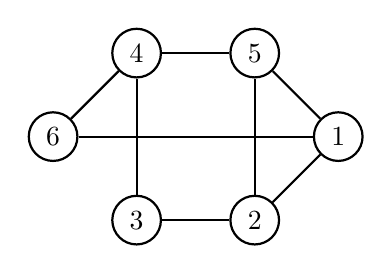
\begin{tikzpicture}[auto,node distance=1.5cm,
 thick,main node/.style={circle,draw}]

  \node[main node] (5) [] {6};
  \node[main node] (2) [below right of=5] {3};
  \node[main node] (3) [above right of=5] {4};
  \node[main node] (4) [right of=3] {5};
  \node[main node] (1) [right of=2] {2};
  \node[main node] (0) [below right of=4] {1};

  \foreach \s/\t in {5/3, 3/4, 4/0, 0/1, 1/2, 2/3, 1/4, 5/0} {
   \path[draw] (\s) edge (\t);}
\end{tikzpicture}
\caption{An undirected graph that is connected.}
\label{fig:example_graph}
\end{figure}

\begin{figure}

 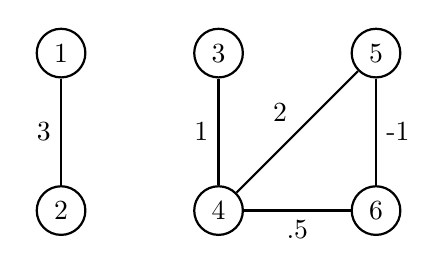
\begin{tikzpicture}[auto,node distance=2cm,
 thick,main node/.style={circle,draw}]

  \node[main node] (0) [] {1};
  \node[main node] (1) [below of=0] {2};
  \node[main node] (2) [right of=0] {3};
  \node[main node] (3) [below of=2] {4};
  \node[main node] (4) [right of=2] {5};
  \node[main node] (5) [right of=3] {6};

   \path[draw] (0) edge node [left] {3} (1);
   \path[draw] (2) edge node [left] {1} (3);
   \path[draw] (4) edge node{-1} (5);
   \path[draw] (3) edge node{2} (4);
   \path[draw] (3) edge node [below]{.5} (5);
\end{tikzpicture}
\caption{A weighted undirected graph that is not connected.}
\label{fig:example_graph2}
\end{figure}

% \begin{tikzpicture}[auto,node distance=1.5cm,
% thick,main node/.style={circle,draw}]
%
%  \node[main node] (2) [] {2};
%  \node[main node] (1) [below left of=2] {1};
%  \node[main node] (0) [below right of=2] {0};
%
%  \foreach \s/\t in {1/1, 1/2, 1/3, 2/3} {
%   \path[draw] (\s) edge (\t);}
%\end{tikzpicture}
%\caption{An undirected graph that is not simple.}
%\label{fig:example_graph}
%\end{figure}


%\begin{figure}
% \begin{tikzpicture}[->,>=stealth',shorten >=1pt,auto,node distance=1.5cm,
% thick,main node/.style={circle,draw}]
%
%  \node[main node] (A) [] {A};
%  \node[main node] (B) [below of=A] {B};
%  \node[main node] (C) [right of=A] {C};
%  \node[main node] (D) [below of=C] {D};
%  \node[main node] (E) [right of=C] {E};
%  \node[main node] (F) [right of=D] {F};
%
%  \foreach \s/\t in {A/C, B/A, B/D, C/E, C/F, D/C} {
%   \path[draw] (\s) edge (\t);}
%\end{tikzpicture}
%\caption{A simple directed graph}
%\end{figure}



Graph theory is a branch of mathematics dealing with mathematical structures called graphs.  Graphs represent relationships between objects.
%For example, the transition diagram in Figure \ref{fig:markov1} in Lab \ref{lab:EigSolve} shows the relationship between states in a Markov chain.
An \emph{undirected graph} is a set of nodes (or vertices) and edges, where each edge connects exactly two nodes (see Figure \ref{fig:example_graph}).
In a \emph{directed graph}, edges are directional. Each edge only goes one way, usually visualized as an arrow pointing from one node to another.
In this lab, we will only consider undirected graphs, which we will simply call graphs (unless we wish to emphasize the fact that they are undirected).

%A graph is \emph{simple} if no edge connects a node to itself. 
%The graph in Figure [TODO!] is simple, but the graph in Figure [TODO!] is not.

A \emph{weighted} graph is a graph with a weight attached to each edge.
For example, a weighted graph could represent a collection of cities with roads connecting them.
The vertices would be cities, the edges would be roads, and weight of an edge would be the length of a road.
Such a graph is depicted in Figure \ref{fig:example_graph2}.

Any unweighted graph can be thought of as a weighted graph by assigning a weight of 1 to each edge.

\subsection*{Adjacency, Degree, and Laplacian Matrices}
We will now introduce three matrices associated with a graph. 
Throughout this section, assume we are working with a weighted undirected graph with $N$ nodes, and that $w_{ij}$ is the weight attached to the edge connecting node $i$ and node $j$.
We first define the adjacency matrix.

\begin{definition} The \emph{adjacency matrix} is an $N \times N$ matrix whose $(i,j)$-th entry is
\begin{center}
	$ \begin{cases}  w_{ij} & \mbox{if an edge connects node i and node j} \\ 0 & \mbox{otherwise.} \end{cases}$
\end{center}
% If the graph is not simple, there are differing conventions for how to define the diagonal of the adjacency matrix.
\end{definition}

For example, the graph in Figure \ref{fig:example_graph} has the adjacency matrix $A_1$ and the graph in Figure \ref{fig:example_graph2} has the adjacency matrix $A_2$, where
\[
A_1 = \begin{pmatrix}
0 & 1 & 0 & 0 & 1 & 1\\
1 & 0 & 1 & 0 & 1 & 0\\
0 & 1 & 0 & 1 & 0 & 0\\
0 & 0 & 1 & 0 & 1 & 1\\
1 & 1 & 0 & 1 & 0 & 0\\
1 & 0 & 0 & 1 & 0 & 0
\end{pmatrix} \qquad A_2 = 
 \begin{pmatrix}
0 & 3 & 0 & 0 & 0 & 0\\
3 & 0 & 0 & 0 & 0 & 0\\
0 & 0 & 0 & 1 & 0 & 0\\
0 & 0 & 1 & 0 & 2 & .5\\
0 & 0 & 0 & 2 & 0 & -1\\
0 & 0 & 0 & .5 & -1 & 0
\end{pmatrix}.
\]
Notice that these adjacency matrices are symmetric. This will always be the case for undirected graphs.

\begin{comment}
Raising the adjacency matrix to a power yields some very interesting information.
We can discover the number of paths of length $n$ between two nodes by raising a graph's adjacency matrix to the $n$th power.
For example, by squaring $A$, we can find the number of paths of length two between every pair of nodes.
\begin{lstlisting}
>>> A = np.array([[0,1,0,0,1,0],[1,0,1,0,1,0],
                  [0,1,0,1,0,0],[0,0,1,0,1,1],
                  [1,1,0,1,0,0],[0,0,0,1,0,0]])

>>> np.linalg.matrix_power(A,2)
array([[2, 1, 1, 1, 1, 0],
       [1, 3, 0, 2, 1, 0],
       [1, 0, 2, 0, 2, 1],
       [1, 2, 0, 3, 0, 0],
       [1, 1, 2, 0, 3, 1],
       [0, 0, 1, 0, 1, 1]])
\end{lstlisting}
We can see that no paths of length two exist between node 0 and node 5 because $A^2_{0,5} = 0$.
By calculating $A^6$ we can find the number of paths of length six from node 3 to itself.
\begin{lstlisting}
>>> np.linalg.matrix_power(A, 6)
array([[45, 54, 38, 45, 54, 16],
       [54, 86, 29, 77, 51, 11],
       [38, 29, 55, 15, 70, 27],
       [45, 77, 15, 75, 31,  4],
       [54, 51, 70, 31, 93, 34],
       [16, 11, 27,  4, 34, 14]])
\end{lstlisting}
We see that there are 75 unique paths of length six from node 3 to itself.
Imagine trying to count all of those paths by hand!
It would be very easy to count incorrectly.
This method makes it very simple to count paths without mistakes.

Adjacency matrices can also be composed of \li{True} and \li{False} values.
In this case, the $n$th power of such a matrix (using boolean arithmetic)
is again a matrix of
boolean values which simply indicate whether there exists a path of length $n$ between the given pair of nodes, rather than indicating the number of such
paths.

\begin{problem}
Let the following matrix represent a directed graph
\[
\begin{pmatrix}
0 & 0 & 1 & 0 & 1 & 0 & 1 \\
1 & 0 & 0 & 0 & 0 & 1 & 0 \\
0 & 0 & 0 & 0 & 0 & 1 & 0 \\
1 & 0 & 0 & 0 & 1 & 0 & 0 \\
0 & 0 & 0 & 1 & 0 & 0 & 0 \\
0 & 0 & 1 & 0 & 0 & 0 & 1 \\
0 & 1 & 0 & 0 & 0 & 0 & 0
\end{pmatrix}
\]
Between which pair of nodes does there exist the greatest number of paths
of length five?
From which node to which node is there no path of length seven?
\end{problem}
\end{comment}

The second matrix is the degree matrix. 
\begin{definition} The \emph{degree matrix} is an $N \times N$ diagonal matrix whose $(i,i)$-th entry is
\[ 
\sum_{j=1}^N w_{ij}.
\]
This quantity is the sum of the weight of each edge leaving node $i$.
\end{definition}
%For a directed graph, each node has an \emph{out-degree} (the number of edges directed away from a node) and an \emph{in-degree} (the number edges directed toward a node).
We call the $(i, i)$-th entry of the degree matrix the \emph{degree} of node $i$. As an example, the degree matrices of the graphs in Figures \ref{fig:example_graph} and \ref{fig:example_graph2} are $D_1$ and $D_2$, respectively.

\[
D_1 = \begin{pmatrix}
3 & 0 & 0 & 0 & 0 & 0\\
0 & 3 & 0 & 0 & 0 & 0\\
0 & 0 & 2 & 0 & 0 & 0\\
0 & 0 & 0 & 3 & 0 & 0\\
0 & 0 & 0 & 0 & 3 & 0\\
0 & 0 & 0 & 0 & 0 & 2
\end{pmatrix}. \qquad D_2 = 
 \begin{pmatrix}
3 & 0 & 0 & 0 & 0 & 0\\
0 & 3 & 0 & 0 & 0 & 0\\
0 & 0 & 1 & 0 & 0 & 0\\
0 & 0 & 0 & 3.5 & 0 & 0\\
0 & 0 & 0 & 0 & 1 & 0\\
0 & 0 & 0 & 0 & 0 & -.5
\end{pmatrix}
\]

Finally, we can combine the degree matrix and the adjacency matrix to get the Laplacian matrix.
% Wikipedia defines the Laplacian of a simple graph only. I don't know why.
% The graph in our application is NOT simple. 
% However, the non-simple parts cancel out, meaning that the Laplacian of the graph is the same as if you removed all self edges and then computed the Laplacian.
% So I just define the Laplacian this way and don't talk about simple graphs.
\begin{definition}
The \emph{Laplacian matrix} of a graph is 
\[D - A \]
where $D$ is the degree matrix and $A$ is the adjacency matrix of the graph.
\end{definition}

For example, the Laplacian matrix of the graphs in Figures \ref{fig:example_graph} and \ref{fig:example_graph2} are $L_1$ and $L_2$, respectively, where

\[
L_1 = \begin{pmatrix}
3 & -1 & 0 & 0 & -1 & -1\\
-1 & 3 & -1 & 0 & -1 & 0\\
0 & -1 & 2 & -1 & 0 & 0\\
0 & 0 & -1 & 3 & -1 & -1\\
-1 & -1 & 0 & -1 & 3& 0\\
-1 & 0 & 0 & -1 & 0 & 2
\end{pmatrix}. \qquad L_2 = 
 \begin{pmatrix}
3 & -3 & 0 & 0 & 0 & 0\\
-3 & 3 & 0 & 0 & 0 & 0\\
0 & 0 & 1 & -1 & 0 & 0\\
0 & 0 & -1 & 3.5 & -2 & -.5\\
0 & 0 & 0 & -2 & 1 & 1\\
0 & 0 & 0 &- .5 & 1 & -.5
\end{pmatrix}
\]

In this lab we will learn about graphs by studying their Laplacian matrices.
While the Laplacian matrix seems simple, we can learn surprising things from its eigenvalues.


\begin{problem}
Write a function that accepts the adjacency matrix of a graph as an argument and returns the Laplacian matrix. 
Test your function on the graphs in Figures \ref{fig:example_graph} and \ref{fig:example_graph2}.

Hint: You can compute the diagonal of the degree matrix in one line by summing over an axis (see Lab \ref{lab:NumpyIntro}).
\label{prob:laplacian}
\end{problem}



\subsection*{Connectivity: First Application of Laplacians}

A \emph{connected graph} is a graph where every vertex is connected to every other vertex by at least one path.
The graph in Figure \ref{fig:example_graph} is connected, whereas the graph in Figure \ref{fig:example_graph2} is not.
It is often important to know if a graph is connected.
A naive approach to determine connectivity of a graph is to search every possible path from each vertex.
While this works for very small graphs, most interesting graphs will have thousands of vertices, and for such graphs this approach is not feasible.

Instead of the naive approach, we can use an interesting result from algebraic graph theory. 
This result relates the connectivity of a graph to its Laplacian.

The Laplacian of any graph always has at least one zero eigenvalue.
Why is this true?  If $L$ is the Laplacian matrix of a graph, then the rows of $L$ must sum to 0.
(Think about how L was created.)
Since this is true, L cannot have full rank, so $\lambda = 0$ must be an eigenvalue of $L$. 

Furthermore, if $L$ represents a graph that is \textit{not} connected, more than one of the eigenvalues of $L$ will be zero. 
To see this, let $J \subset \{1 \dots N\}$ such that the vertices $\{v_j\}_{j \in J}$ form a connected component of the graph. 
Define a vector $\x$ such that
 \[
    \x_j = \begin{cases}
        1, & j \in J \\
        0, & j \not\in J
        \end{cases}
  \]

Then $\x$ is an eigenvector of $L$ corresponding to the eigenvalue $\lambda = 0$. 
(Look at the Laplacian matrix in Figure \ref{fig:example_graph2} and consider the product $L_2 \x$.) 
In other words, for each connected component, 0 appears at least once as an eigenvalue.

In fact, it can be rigorously proven that the number of zero eigenvalues of the Laplacian exactly \textit{equals} the number of connected components. 
If we can solve for the eigenvalues of $L$, this makes it simple to calculate how many connected components are in the graph.

$L$ is always a positive semi-definite matrix, so all of its eigenvalues are greater than or equal to 0.
The second smallest eigenvalue of $L$ is known as the \textit{algebraic connectivity} of the graph.
It is clearly 0 for non-connected graphs.
For connected graphs, the algebraic connectivity can give us useful information about the sparsity or ``connectedness'' of a graph.
A higher algebraic connectivity indicates that the graph is more strongly connected.

\begin{comment}
Thus, it will have real eigenvalues. 
Surprisingly, a graph is connected if the second smallest eigenvalue of its Laplacian matrix is positive.  By second smallest, we mean the second eigenvalue when they are ordered smallest to largest.  The eigenvalues of the Laplacian matrix are never negative; thus, if the second one is not zero, the graph is connected.
In many applications, the Laplacian matrix is sparse, so by taking advantage of this sparsity, we can cheaply determine if a graph is connected.
\end{comment}

\begin{problem}
\leavevmode
Compute the number of connected components in a graph.
Write a function that accepts the adjacency matrix of a graph and returns two arguments: the number of connected components, and the algebraic connectivity of the graph (second smallest eigenvalue of the Laplacian).

Use the \li{scipy.linalg} package to compute the eigenvalues.
Note that this package will return complex eigenvalues (with negligible imaginary parts). Keep only the real parts.
Your function should also accept a tolerance value, such that all eigenvalues less than this value are assumed to be zero.
This should default to \li{tol=1e-8}.

\begin{comment}
%Old part of problem, removed because no great way to evaluate it
Here is a function that creates a random symmetric matrix of Boolean values with sparsity determined by the input \li{c}.
\begin{lstlisting}
def sparse_generator(n, c):
    ''' Return a symmetric nxn matrix with sparsity determined by c.
    Inputs:
        n (int): dimension of matrix
        c (float): a float in [0,1]. Larger values of c will produce
             matrices with more entries equal to zero.
    '''
    A = np.random.rand(n**2).reshape((n, n))
    A = ( A > c**(.5) )
    return A.T.dot(A)
\end{lstlisting}

Test your function on matrices created by \li{sparse_generator} with inputs $n = 10, 100$ and $c = .25, .5, .95$. 
What do you notice about the likelihood that a random graph is connected?
\end{comment}

\end{problem}


\section*{Image Segmentation: Second Application of Laplacians}

\begin{figure}
    \centering
    \begin{subfigure}{0.31\textwidth}
        
\includegraphics[width=\textwidth]{RegMon.png}
    \end{subfigure}
   \hspace*{\fill}
    \begin{subfigure}{0.31\textwidth}
        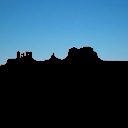
\includegraphics[width=\textwidth]{NegMon.png}
    \end{subfigure}
    \hspace*{\fill}
    \begin{subfigure}{0.31\textwidth}
        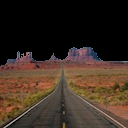
\includegraphics[width=\textwidth]{PosMon.png}
    \end{subfigure}
    
\caption{An image and its segments.}
\label{fig:monument}
\end{figure}
Image segmentation is the process of finding natural boundaries in an image (see Figure \ref{fig:monument}).
This is a simple task for humans, who can easily pick out portions of an image that ``belong together.''
In this lab, you will learn one way for a computer to segment images using graph theory.

The algorithm we will present comes from a paper by Jianbo Shi and Jitendra Malik in 2000 (\cite{Shi2000}).
They segment an image using the following steps.
\begin{enumerate}
	\item \textbf{Represent the image as a weighted graph of pixels.} 
An image is made up of individual pixels, each having a brightness and a location.
(Here, \emph{brightness} is equivalent to the grayscale value of the pixel.)
To define a graph representing the image, we let each pixel be a vertex.
%We say that two pixels are connected in the graph if they are close together, i.e. within some distance $r$ of each other, in the image.
The weight of the edges between two pixels is determined by their distance apart and their similarity in brightness.
We define the graph so that two similar pixels (i.e., with similar brightness and location) will be connected by a strong edge.
	\item \textbf{Calculate the Laplacian.} 
We calculate the adjacency and degree matrices of the graph representing the image, and use these to obtain the Laplacian.
	\item \textbf{Choose the best cut.} 
The graph we have created is connected, but not all edges have the same weight.
Dissimilar pixels will be connected by edges that have a low weight.
We can split the graph into two connected components by ``cutting" it along the low-weight edges.
These components are the image segments we are looking for.
(We can also cut an image multiple times to segment it into more than two pieces.)
As we will see later, Shi and Malik's algorithm uses spectral information (eigenvectors) of the Laplacian to minimize the weight of the cut edges.
\end{enumerate}

\begin{comment}
% Previous explanation which was refactored into the list form above
Their idea is to represent an image as a weighted graph as follows. 
To a computer, an \emph{image} is a collection of \emph{pixels}. 
Each pixel has a brightness and coordinates describing its location in the image.
To define a graph representing this image, we let every pixel be a vertex.
Two pixels are connected if the distance between their coordinates is small (less than $r$).
The weight of the edge connecting two pixels is related to their similarity in brightness, where a low weight means they are very different.

After defining this graph, we will segment the image by ``cutting'' (or removing) edges with low weights, which represent lines of high contrast in the image. 
The ``cut'' is the total weight of the edges removed. Thus, to segment an image, we wish to minimize the ``cut.''
We can ``cut'' an image multiple times to segment an image into more than two pieces.
\end{comment}


\subsection*{Defining the Graph and Adjacency Matrix}

%New
We now define the graph that represents an image. In our $M \times N$ image, the associated graph will have $MN$ nodes, one representing each pixel. We let $w_{ij}$ be the weight of the edge connecting pixels $i$ and $j$, and define

 \begin{equation}
 \label{eq:adjacency}
w_{ij} = \begin{cases} \exp(-\frac{|I(i) - I(j)|}{\sigma_I^2}-\frac{d(i,j)}{\sigma_d^2}) & \mbox{ for $d(i,j) < r$} \\ 0 & \mbox{ otherwise,} \end{cases}
\end{equation}
where
\begin{itemize}
	\item$d(i,j)$ is the Euclidean distance between pixel $i$ and pixel $j$
	\item $|I(i) - I(j)|$ is the difference in brightness of pixels $i$ and $j$
	\item $r$, $\sigma_I$ and $\sigma_d$ are constants that we choose
\end{itemize}

With this definition, pixels that are farther apart than radius $r$ will never be connected. 
Pixels within $r$ will be strongly connected if they are similar in brightness ($|I(i) - I(j)|$ is small) and close together ($d(i,j)$ is small).
Highly contrasting pixels ($|I(i) - I(j)|$ is large) will be weakly connected. 
This gives us a graph with the properties that we intuitively want.

The adjacency matrix $W$ is $(MN) \times (MN)$ and has $w_{ij}$ as its $ij$th entry. 
$W$ will be sparse as long as $r$ is small. 
Figure \ref{fig:adjacency} shows a visualization of the adjacency matrix for a $4 \times 4$ image when $r=1.2$.

\begin{comment}
Now let us define the adjacency matrix of the graph associated to an image. 
Since an $M \times N$ image has $M \times N$ pixels, the adjacency matrix will be $(M \times N) \times (M \times N)$.
After choosing a radius $r$ and some scaling factors $\sigma_I$ and $\sigma_d$, we define the adjacency matrix to be $W = (w_{ij})$, where

\begin{equation}
\label{eq:adjacency}
w_{ij} = \begin{cases} \exp(-\frac{|I(i) - I(j)|}{\sigma_I^2}-\frac{d(i,j)}{\sigma_d^2}) & \mbox{ for $d(i,j) < r$} \\ 0 & \mbox{ otherwise,} \end{cases}
\end{equation}
where
\begin{itemize}
	\item$d(i,j)$ is the Euclidean distance between pixel $i$ and pixel $j$.
	\item $|I(i) - I(j)|$ is the difference in brightness of pixels $i$ and $j$.
\end{itemize}

$W$ will be sparse as long as $r$ is small. 
Figure \ref{fig:adjacency} shows what the adjacency matrix looks like for a $4x4$ image when $r=1.2$.
\end{comment}

\begin{figure}
\begin{tikzpicture}[dot/.style={circle,fill=black,minimum 
	size=4pt,inner sep=0pt,outer sep=-1pt}, >=stealth]
%scale=.85, transform shape,


%image
\draw[step=.75,thick](2.999,0)grid(6,3);
%numbers 1-16
\foreach \x in {1,2,3,4}
	\foreach \y in {4}
		\node[draw=none, anchor=south west]at(\x*.75+2.6, \y-1.4){\x};
\foreach \x [evaluate=\x as \r using int(\x+4)]in {1,2,3,4}
	\foreach \y in {3}
		\node[draw=none, anchor=south west]at(\x*.75+2.6, \y-1.2){\r};
\foreach \x [evaluate=\x as \r using int(\x+8)] in {1,2,3,4}
	\foreach \y in {2}
		\node[draw=none, anchor=south west]at(\x*.75+2.5, \y-.95){\r};
\foreach \x [evaluate=\x as \r using int(\x+12)] in {1,2,3,4}
	\foreach \y in {1}
		\node[draw=none, anchor=south west]at(\x*.75+2.5, \y-.7){\r};

\node[draw=none](image)at(4.5, -.5){$image$};
\node[draw=none](flattened)at(7.25,-3){\textit{flattened image}};
\node[draw=none](adjacency)at(12,-3){\textit{adjacency matrix}};

%dots within grid
\foreach \x in {1,2,3,4}
	\foreach \y in {1,2,3,4}
		\node[draw, dot]at(\x*.75+2.6,\y*.75-.4){};

%color fill
\foreach \x/\y in {2/3.75, 1.25/3, 2/3, 2.75/3, 2/2.25} {\node[draw, minimum 
	size=.75cm, fill=green!30!black, fill opacity=.25]at(\x+2.118,\y-1.118){};}

%circle in image
\node[draw, circle, minimum size=2cm,thick](circle)at(4.13,1.86){};

%flattened image
\draw[step=.5, thick](6.999,-2.5)grid(7.5,5.5);
\foreach \x in {7}
	\foreach \y in {1,...,16}
		\node[draw=none]at(\x+.25,\y*-.5+5.75){\y};

\draw[->,thick](6.1, 1.5)--(6.9,1.5);

%adjancey matrix
\draw[step=.5](7.9999,-2.5)grid(16,5.5);
%\draw[step=2,thick](7.999,-2.5)grid(16,5.5);

%outside labels
\foreach \x in {1,5,9,13} {\node[draw=none]at(\x*.5+7.75,5.8){\x};}
\foreach \y in {1,5,9,13}{\node[draw=none]at(16.3,\y*-.5+5.8){\y};}

%shading of boxes
\foreach \x/\y in {8.5/5.5, 9/5.5, 8.5/5, 9/5, 9.5/5,9/4.5,9.5/4.5,10/4.5, 
	9.5/4, 10/4, 10.5/5.5, 11/5,11.5/4.5, 12/4, 12.5/3.5, 
	13.5/2.5, 14/2, 14.5/1.5, 15/1, 15.5/.5,16/0, 10.5/3.5, 11/3.5, 11/2.5, 
	11.5/2.5,12/2.5, 11.5/2,12/2, 12.5/1.5, 13/1.5, 12.5/1, 13/1,
	13.5/1,13/.5,13.5/.5,14/.5, 13.5/0,14/0, 14.5/-.5,15/-.5,14.5/-1,
	15/-1,15.5/-1, 15/-1.5, 15.5/-1.5, 16/-1.5, 15.5/-2, 16/-2, 8.5/3.5,
	9.5/2.5,10/2,10.5/1.5,11/1,11.5/.5,12/0, 12.5/-.5, 13/-1, 13.5/-1.5, 14/-2} 
	{\node[draw, minimum size=.5cm, fill=black, fill opacity=.25]
	at(\x-.25,\y-.25){};}

%green shaded boxes
\foreach \x/\y in {9/3,11/3, 11.5/3, 10.5/3, 13/3} {\node
	[draw, minimum size=.5cm, fill=shadecolor]
	at(\x-.25,\y-.25){};}

\node[draw=none]at(8.75,2.75){2};
\node[draw=none]at(10.25,2.75){5};
\node[draw=none]at(10.75,2.75){6};
\node[draw=none]at(11.25,2.75){7};
\node[draw=none]at(12.75,2.75){10};

\end{tikzpicture}

\caption{The grid on the left represents a $4\times4$ (or $M \times N$) image with 16 pixels. 
At right is the corresponding $16 \times 16$ (or $(MN) \times (MN)$) adjacency matrix with all nonzero entries shaded.
For example, in the $6^{th}$ row, entries 2, 5, 6, 7, and 10 are nonzero because those pixels are within radius $r$ of pixel 6 (here $r = 1.2$).}
%For example, the $6^{th}$ row corresponds to the $6^{th}$ pixel. 
%Within that row, entries are nonzero if they correspond to pixels that are within radius $r$ of pixel 6 ($r = 1.2$ was used here).}
\label{fig:adjacency}
\end{figure}


\subsection*{Computing the Adjacency Matrix}
We will now write a function to compute the adjacency matrix for a given image.
%The function will also accept constants \li{radius}, \li{sigma_I}, and \li{sigma_d} to use in \ref{eq:adjacency}. 
The function will accept a filename and constants \li{radius}, \li{sigma_I}, and \li{sigma_d}, and return the adjacency matrix and the diagonal of the corresponding degree matrix. 

The basic approach is straightforward. 
For each pixel in the image, compare it to every other pixel, use (\ref{eq:adjacency}) to calculate the weight of the edge between them, and fill in the weight in the adjacency matrix.
This section will discuss how to implement this efficiently in Python.

First, load an image and convert it to grayscale. 
The included function \li{getImage} helps handle color images.
It accepts a filename and returns a 2-D grayscale image.

It will be useful to flatten the $M \times N$ image.
This converts it into a 1-D array of pixels of length $MN$, essentially giving each pixel an index. 
We can use \li{img.flatten} to flatten the array \li{img}.
\begin{lstlisting}
>>> A = np.array([[1,2],[3,4]])
>>> A.flatten()                
array([1,2,3,4])
\end{lstlisting}

Next, initialize empty adjacency and degree matrices to fill in. 
As in Figure \ref{fig:adjacency}, the adjacency matrix will be sparse, so initialize it as a sparse matrix \li{W}. 
Use the sparse matrix type \li{lil_matrix}, which is optimized for filling in a matrix one entry at a time. 
Since we only need to store the diagonal of the degree matrix, initialize this diagonal as a regular 1-dimensional NumPy array \li{D}.

We now fill in \li{W} according to our definition in Equation \ref{eq:adjacency}.
Each pixel in the image corresponds to one row in \li{W}.
For each pixel:
\begin{itemize}
\item Find its neighbors (the pixels in the image that are within distance $r$ of it)
\item Use \ref{eq:adjacency} to calculate the weights connecting the pixel to each of its neighbors
\item Fill in these weights in \li{W}, leaving the rest of the values in the row as zeros. \footnote{Note that \li{W} will be a symmetric matrix. We could potentially speed up this algorithm by taking advantage of this fact.}
\end{itemize} 
The sum of the entries of a row in \li{W} will be the corresponding entry in \li{D}. 

You may choose to use the provided helper function \li{getNeighbors} to find the neighbors of a given pixel.
The function accepts the index of a pixel in the flattened image, along with a value for $r$ and the original image dimensions. 
It returns two flat arrays: \li{indices} and \li{distances}. 
The array \li{indices} contains the indices of the neighbor pixels within distance $r$ of the input pixel. 
The array \li{distances} contains the corresponding distances of those pixels from the input pixel.
%According to (\ref{eq:adjacency}), the array \li{indices} contains exactly the indices of the nonzero entries of the current row of \li{W}.  
Using Figure \ref{fig:adjacency} as an example, with the inputs 6, 1.2, 4, and 4 the outputs would be \li{indices = array([2,5,6,7,10])} and \li{distances = array([1,1,0,1,1])}. 
Try running the function with different inputs to build intuition about what it does.

Finally, convert \li{W} to the sparse matrix type \li{csc_matrix}, which is faster for computations. Then return \li{W} and \li{D}.

\begin{problem}
Write the function \li{adjacency} described in this section.
Accept an image a filename and constants \li{radius}, \li{sigma_I}, and \li{sigma_d}.
Return the corresponding sparse adjacency matrix \li{W} and the diagonal of the degree matrix \li{D}.
Use (\ref{eq:adjacency}) to compute the weights in the adjacency matrix.
For speed, try to compute an entire row of \li{W} at once, instead of filling in \li{W} entry by entry.


%Notice that for each pixel you can save time by only checking the pixels $r$ rows and columns away.
%For that you'll have to handle the pixels on the edges and corners of the image carefully.
%I gave them new helper code, which abstracts away the edge cases.
\label{prob:adjacency_dream}
\end{problem}

\subsection*{Minimizing the `Cut'}
As stated earlier, the goal is to split the image into two segments, while minimizing the weight of the edges that are `cut' in the corresponding graph.
Let $L$ be the Laplacian of the adjacency matrix defined in \ref{eq:adjacency} and let $D$ be the degree matrix.
Shi and Malik proved that using the second smallest eigenvalue of $D^{-1/2}LD^{-1/2}$, we can minimize the `cut' .
Both $D$ and $L$ will be symmetric matrices, so all eigenvalues of $D^{-1/2}LD^{-1/2}$ will be real, therefore the second smallest one is well-defined.
(Note that $D^{-1/2}$ refers not to matrix, but element-wise, exponentiation.)

The eigenvector associated to the second smallest eigenvalue is the key to segmenting the image. 
This eigenvector will have $MN$ entries.
Shi and Malik proved that the indices of its \emph{positive} entries are the indices of the pixels in the flattened image which belong in one segment.
Likewise, the indices of its \emph{negative} entries are the indices of the pixels which belong in the other segment.

To compute the segments, reshape this eigenvector as an $M \times N$ array, and set the positive entries to True and the negative entries to False.
We can multiply this True-False mask entry-wise by the image. 
This zeros out the pixels in the image corresponding to the \li{False} entries in the mask, without affecting the pixels corresponding to \li{True} entries. 
We can negate the mask using the tilde operator, which lets us compute the other segment of the image. 
Finally we return the two segments.

\begin{comment}
Here is the definition of a function that will segment an image.
\begin{lstlisting}
1. def segment(img):
\end{lstlisting}

Use the function \li{adjacency} from Problem \ref{prob:adjacency_dream} to compute the adjacency matrix and the diagonal of the degree matrices of the image.
\begin{lstlisting}
2.     W, D = adjacency(img)
\end{lstlisting}

Next we create sparse matrices corresponding to $D$ and $D^{-1/2}$ in Shi and Malik's algorithm. Remember that the sparse matrix type \li{csc_matrix} is best for computations.
\begin{lstlisting}
3.     Dsq = # calculate the square root of D
4.     D_matrix = spar.spdiags(D, 0, D.shape[1], D.shape[1], format = 'csc')
5.     Dsq_matrix = # create a sparse matrix with diagonal Dsq
\end{lstlisting}
Now it is simple to compute $D^{-1/2}LD^{-1/2}$. We call this matrix \li{P}.
\begin{lstlisting}
6.     L = # compute the Laplacian
7.     P = # compute D^{-1/2}*L*D^{-1/2} as in Shi and Malik's algorithm
\end{lstlisting}
According to Shi and Malik, we need the eigenvector corresponding to the second smallest eigenvalue of \li{P}. We compute this with the \li{eigs()} method of the \li{scipy.sparse.linalg} module. We set the parameter \li{which='SR'} in the function call in order to compute the eigenvalues with Smallest Real part and their corresponding eigenvectors. The parameter \li{k} in the function call can be used to specify how many eigenvalues the method computes.
\begin{lstlisting}
8.     e = # compute the two smallest eigenvalues of P and their eigenvectors
9.     eigvec = # eigenvector of the second smallest eigenvalue
\end{lstlisting}

Next we create a mask that is \li{True} wherever \li{eigvec} is positive and reshape it to be the size of \li{img}. 
\begin{lstlisting}
10.    mask = # create mask
\end{lstlisting}

\begin{lstlisting}
11.    pos = # compute positive segment
12.    neg = # compute negative segment
13.    return pos, neg
\end{lstlisting}

\end{comment}

\begin{problem} Write the function \li{segment} to segment an image.
The function should accept an image filename and return both of the segments.
You should call the code you wrote in Problem \ref{prob:adjacency_dream}.
Use sparse matrices where possible.


Test on the image \li{dream.png}.
Your segments should look like the segments in Figure \ref{fig:dream_solution} (the original image is on the left). 

Hints:
\begin{enumerate}
\item After defining $D^{-1/2}$, convert $D$ and $D^{-1/2}$ into sparse matrices using \li{scipy.sparse.spdiags}.
\item Since are now dealing with sparse instead of dense matrices, you shouldn't use your solution to Problem \ref{prob:laplacian} to calculate the Laplacian. 

\item Multiply sparse matrices with \li{A.dot(B)}.

\item Use \li{scipy.sparse.eigsh} to calculate the eigenvector. This is a sparse eigenvalue solver optimized for symmetric matrices.
Set the keyword \li{which = "SM"} to return the smallest eigenvalues.

\item The provided function \li{displayPosNeg} can be used to plot your images. 

\end{enumerate}

\end{problem}

\begin{figure}
\centering
    \centering
    \begin{subfigure}{0.31\textwidth}
        
\includegraphics[width=\textwidth]{RegDream.png}
    \end{subfigure}
    \hspace*{\fill}
    \begin{subfigure}{0.31\textwidth}
        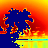
\includegraphics[width=\textwidth]{NegDream.png}
    \end{subfigure}
    \hspace*{\fill}
    \begin{subfigure}{0.31\textwidth}
        
\includegraphics[width=\textwidth]{PosDream.png}
    \end{subfigure}
\caption{Segments of \li{dream.png}}
\label{fig:dream_solution}
\end{figure}

\begin{comment} %Old stuff from middle of lab
Here is the function definition, which includes some default values for the constants.
\begin{lstlisting}
1.	def adjacency(img, radius=5.0, sigma_I = .15, sigma_d = 1.7):
\end{lstlisting}
\begin{lstlisting}
4.     W = spar.lil_matrix((flat_img.size, flat_img.size), dtype=float)
5.     D = np.zeros((1, flat_img.size))
\end{lstlisting}

Later, our function will iterate through the rows of the adjacency matrix, initializing one row at a time. Each row corresponds to a pixel of the original image. Thus, we begin by flattening the image (see Figure \ref{fig:adjacency}). We also store the dimensions of \li{img} for later.
\begin{lstlisting}
2.     flat_img = img.flatten()
3.     height, width = img.shape
\end{lstlisting}

\begin{lstlisting}
6.     for pixel in xrange(flat_img.size):
7.         indices, distances = getNeighbors(pixel, radius, height, width)
8.         weights = # weights[j] should be W[pixel, indices[j]]
9.         W[pixel, indices] = weights
10.        D[0,pixel] = weights.sum()
\end{lstlisting}
\end{comment}

\begin{comment}
\begin{lstlisting}
11.    W = W.tocsc()
12.    return W, D
\end{lstlisting}
\end{comment}

\begin{comment}
\section*{Appendix: helper code for Problem \ref{prob:adjacency_dream}}
Here is the function \li{getNeighbors} which you can use to compute the adjacency matrix of an image, as in Problem \ref{prob:adjacency_dream}.

\lstinputlisting[style=fromfile]{getNeighbors.py}
\end{comment}